% Libertad gauge: diferentes marcos locales en una superficie
% Compilar con: pdflatex gauge_freedom.tex
\documentclass[tikz,border=10pt]{standalone}
\usepackage[T1]{fontenc}
\usepackage[utf8]{inputenc}
\usepackage{tikz}
\usepackage{amsmath,amssymb}
\usetikzlibrary{arrows.meta, calc}

\definecolor{gdlblue}{RGB}{41, 98, 168}
\definecolor{gdlred}{RGB}{191, 49, 49}
\definecolor{gdlgreen}{RGB}{30, 130, 76}
\definecolor{gdlorange}{RGB}{217, 130, 30}
\definecolor{gdlpurple}{RGB}{118, 56, 138}
\definecolor{gdlgray}{RGB}{140, 140, 140}
\definecolor{gdlyellow}{RGB}{190, 140, 10}

\begin{document}
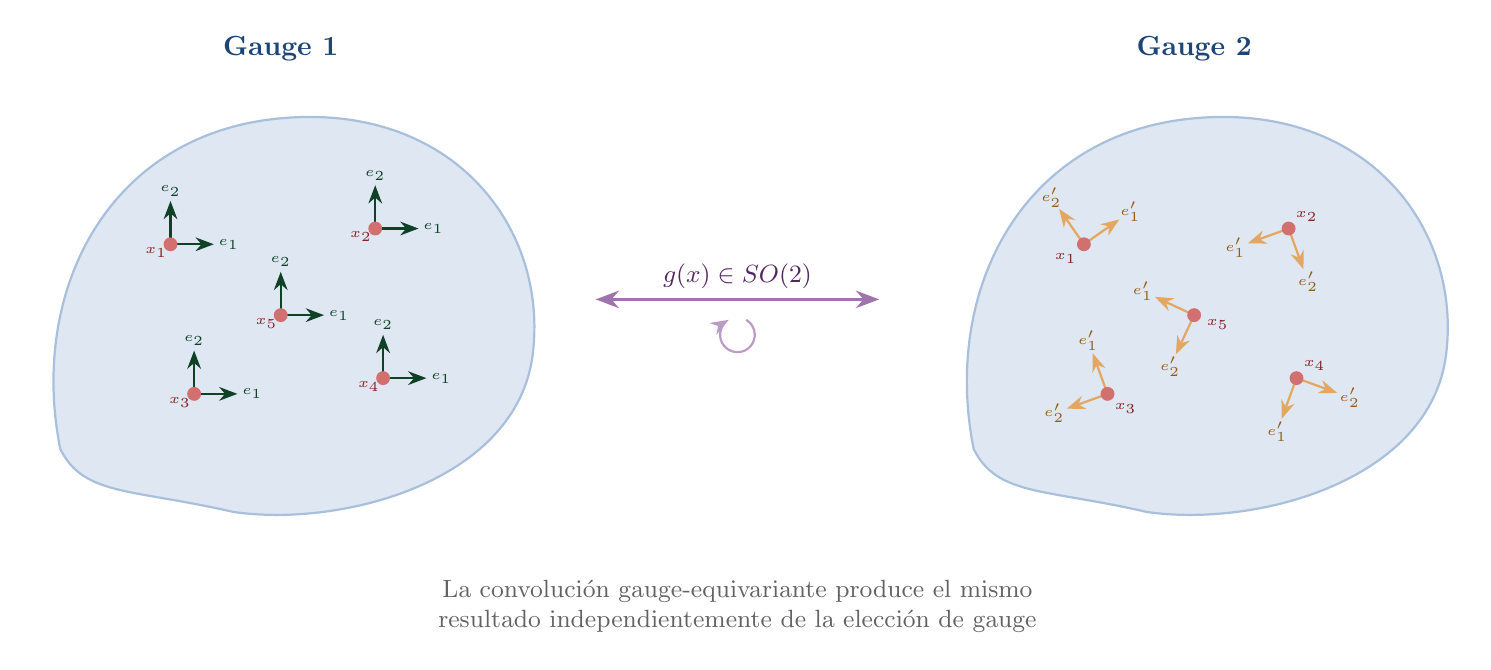
\begin{tikzpicture}[>=Stealth]

% =============================================
% Surface shape macro (reusable for both panels)
% A generous blob giving ~1cm margin for arrows
% =============================================
\def\surfacepath{
    (-2.8, -1.4) .. controls (-3.2, 0.6) and (-2.2, 2.6) .. (0, 2.8)
    .. controls (2.2, 3.0) and (3.4, 1.4) .. (3.2, -0.2)
    .. controls (3.0, -1.8) and (0.8, -2.4) .. (-0.6, -2.2)
    .. controls (-1.9, -1.9) and (-2.5, -2.0) .. (-2.8, -1.4)
}

% Arrow length for local frames
\newcommand{\framelen}{0.55}
% Label distance from arrow tip
\newcommand{\laboff}{0.17}

% =============================================
% Gauge 1 (left): consistent orientation
% =============================================
\begin{scope}[shift={(-5.8, 0)}]
    \node[above, font=\bfseries, text=gdlblue!70!black] at (0, 3.4) {Gauge 1};

    % Surface
    \fill[gdlblue!15] \surfacepath;
    \draw[thick, gdlblue!40] \surfacepath;

    % 5 well-separated points (kept away from edges)
    \coordinate (p1) at (-1.4, 1.2);
    \coordinate (p2) at (1.2, 1.4);
    \coordinate (p3) at (-1.1, -0.7);
    \coordinate (p4) at (1.3, -0.5);
    \coordinate (p5) at (0.0, 0.3);

    % All frames consistently oriented: e1 = right, e2 = up
    \foreach \p in {p1, p2, p3, p4, p5} {
        \draw[->, thick, gdlgreen!50!black] (\p) -- ++(0:\framelen);
        \draw[->, thick, gdlgreen!50!black] (\p) -- ++(90:\framelen);
        \fill[gdlred!70] (\p) circle (2.5pt);
    }

    % e1 labels
    \foreach \p in {p1, p2, p3, p4, p5} {
        \node[font=\tiny, gdlgreen!50!black, right, inner sep=1pt]
            at ($(\p)+(0:\framelen)+(0.02,0)$) {$e_1$};
    }
    % e2 labels
    \foreach \p in {p1, p2, p3, p4, p5} {
        \node[font=\tiny, gdlgreen!50!black, above, inner sep=1pt]
            at ($(\p)+(90:\framelen)+(0,0.02)$) {$e_2$};
    }

    % Point labels (below-left of each dot, away from arrows)
    \node[font=\tiny, below left, text=gdlred!70!black, inner sep=1pt] at (p1) {$x_1$};
    \node[font=\tiny, below left, text=gdlred!70!black, inner sep=1pt] at (p2) {$x_2$};
    \node[font=\tiny, below left, text=gdlred!70!black, inner sep=1pt] at (p3) {$x_3$};
    \node[font=\tiny, below left, text=gdlred!70!black, inner sep=1pt] at (p4) {$x_4$};
    \node[font=\tiny, below left, text=gdlred!70!black, inner sep=1pt] at (p5) {$x_5$};
\end{scope}

% =============================================
% Gauge 2 (right): different orientations per point
% =============================================
\begin{scope}[shift={(5.8, 0)}]
    \node[above, font=\bfseries, text=gdlblue!70!black] at (0, 3.4) {Gauge 2};

    % Surface (same shape)
    \fill[gdlblue!15] \surfacepath;
    \draw[thick, gdlblue!40] \surfacepath;

    % Same point positions
    \coordinate (q1) at (-1.4, 1.2);
    \coordinate (q2) at (1.2, 1.4);
    \coordinate (q3) at (-1.1, -0.7);
    \coordinate (q4) at (1.3, -0.5);
    \coordinate (q5) at (0.0, 0.3);

    % Frame at q1: rotated 35 deg
    \draw[->, thick, gdlorange!70] (q1) -- ++(35:\framelen);
    \draw[->, thick, gdlorange!70] (q1) -- ++(125:\framelen);
    \fill[gdlred!70] (q1) circle (2.5pt);
    \node[font=\tiny, gdlorange!70!black] at ($(q1)+(35:\framelen+\laboff)$) {$e_1'$};
    \node[font=\tiny, gdlorange!70!black] at ($(q1)+(125:\framelen+\laboff)$) {$e_2'$};

    % Frame at q2: rotated 200 deg (e1 points lower-left, e2 points upper-left)
    \draw[->, thick, gdlorange!70] (q2) -- ++(200:\framelen);
    \draw[->, thick, gdlorange!70] (q2) -- ++(290:\framelen);
    \fill[gdlred!70] (q2) circle (2.5pt);
    \node[font=\tiny, gdlorange!70!black] at ($(q2)+(200:\framelen+\laboff)$) {$e_1'$};
    \node[font=\tiny, gdlorange!70!black] at ($(q2)+(290:\framelen+\laboff)$) {$e_2'$};

    % Frame at q3: rotated 110 deg
    \draw[->, thick, gdlorange!70] (q3) -- ++(110:\framelen);
    \draw[->, thick, gdlorange!70] (q3) -- ++(200:\framelen);
    \fill[gdlred!70] (q3) circle (2.5pt);
    \node[font=\tiny, gdlorange!70!black] at ($(q3)+(110:\framelen+\laboff)$) {$e_1'$};
    \node[font=\tiny, gdlorange!70!black] at ($(q3)+(200:\framelen+\laboff)$) {$e_2'$};

    % Frame at q4: rotated 250 deg (pointing mostly down-left and up-left)
    \draw[->, thick, gdlorange!70] (q4) -- ++(250:\framelen);
    \draw[->, thick, gdlorange!70] (q4) -- ++(340:\framelen);
    \fill[gdlred!70] (q4) circle (2.5pt);
    \node[font=\tiny, gdlorange!70!black] at ($(q4)+(250:\framelen+\laboff)$) {$e_1'$};
    \node[font=\tiny, gdlorange!70!black] at ($(q4)+(340:\framelen+\laboff)$) {$e_2'$};

    % Frame at q5: rotated 155 deg
    \draw[->, thick, gdlorange!70] (q5) -- ++(155:\framelen);
    \draw[->, thick, gdlorange!70] (q5) -- ++(245:\framelen);
    \fill[gdlred!70] (q5) circle (2.5pt);
    \node[font=\tiny, gdlorange!70!black] at ($(q5)+(155:\framelen+\laboff)$) {$e_1'$};
    \node[font=\tiny, gdlorange!70!black] at ($(q5)+(245:\framelen+\laboff)$) {$e_2'$};

    % Point labels (positioned to avoid overlapping with rotated arrows)
    \node[font=\tiny, below left, text=gdlred!70!black, inner sep=1pt] at ($(q1)+(-0.05,-0.08)$) {$x_1$};
    \node[font=\tiny, above right, text=gdlred!70!black, inner sep=1pt] at ($(q2)+(0.05,0.05)$) {$x_2$};
    \node[font=\tiny, below right, text=gdlred!70!black, inner sep=1pt] at ($(q3)+(0.05,-0.08)$) {$x_3$};
    \node[font=\tiny, above right, text=gdlred!70!black, inner sep=1pt] at ($(q4)+(0.05,0.05)$) {$x_4$};
    \node[font=\tiny, right, text=gdlred!70!black, inner sep=1pt] at ($(q5)+(0.12,-0.12)$) {$x_5$};
\end{scope}

% =============================================
% Double arrow between surfaces (gauge transformation)
% =============================================
\draw[<->, very thick, gdlpurple!70] (-1.8, 0.5) --
    node[above, font=\small, text=gdlpurple!70!black] {$g(x) \in SO(2)$}
    (1.8, 0.5);

% Rotation arc icon below the label
\draw[gdlpurple!50, thick, ->] (0, 0.05) ++(60:0.22) arc (60:-240:0.22);

% =============================================
% Caption text below
% =============================================
\node[font=\small, text width=13cm, align=center, text=gdlgray!70!black] at (0, -3.4) {
    La convolución gauge-equivariante produce el mismo resultado
    independientemente de la elección de gauge
};

\end{tikzpicture}
\end{document}
